\documentclass[tikz,border=6pt]{standalone}
\usepackage{pgfplots}
\pgfplotsset{compat=1.18}
\begin{document}
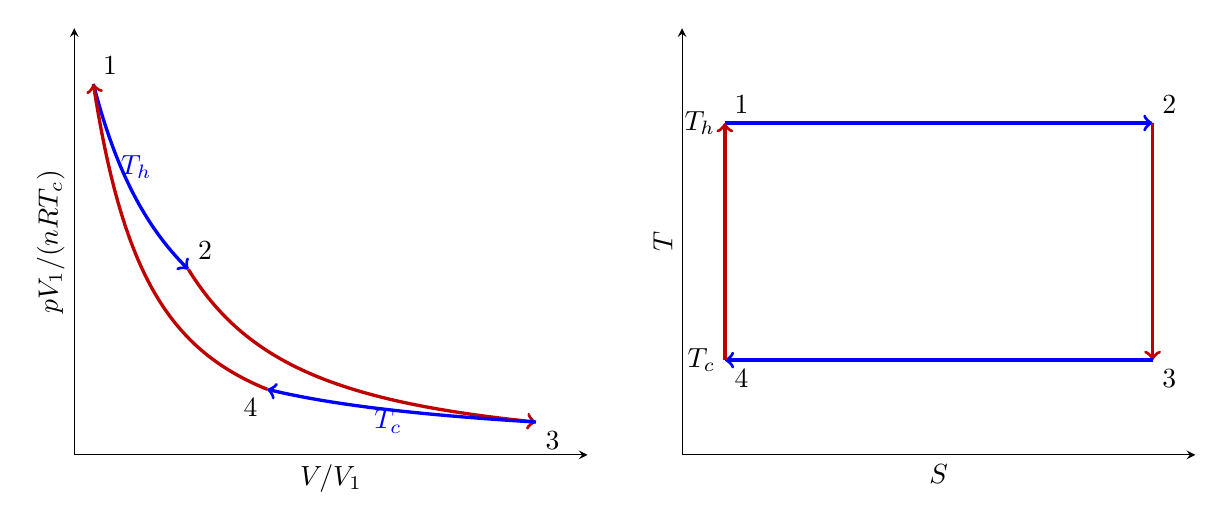
\begin{tikzpicture}
\begin{axis}[
 name=pv,width=8.1cm,height=7cm,axis lines=left,
 xlabel={$V/V_1$},ylabel={$pV_1/(nRT_c)$},
 xmin=.8,xmax=6.2,ymin=0,ymax=2.3,
 ticks=none,clip=false]
% Exact dimensionless example: Th/Tc=2, gamma=5/3, V2/V1=2.
% The adiabatic volume multiplier is (Th/Tc)^(1/(gamma-1))=2^(3/2).
% Hence V3/V1=2^(5/2)=5.656854 and V4/V1=2^(3/2)=2.828427.
\addplot[very thick,blue,domain=1:2,samples=100,->] {2/x};
\addplot[very thick,red!75!black,domain=2:5.656854,samples=160,->]
  {2^(5/3)/x^(5/3)};
\addplot[very thick,blue,domain=2.828427:5.656854,samples=100,<-] {1/x};
\addplot[very thick,red!75!black,domain=1:2.828427,samples=140,<-]
  {2/x^(5/3)};
\node[anchor=south west] at (axis cs:1,2) {$1$};
\node[anchor=south west] at (axis cs:2,1) {$2$};
\node[anchor=north west] at (axis cs:5.656854,.17678) {$3$};
\node[anchor=north east] at (axis cs:2.828427,.35355) {$4$};
\node[blue] at (axis cs:1.45,1.55) {$T_h$};
\node[blue] at (axis cs:4.1,.18) {$T_c$};
\end{axis}
\begin{axis}[
 at={(pv.east)},anchor=west,xshift=1.2cm,
 width=8.1cm,height=7cm,axis lines=left,
 xlabel={$S$},ylabel={$T$},xmin=-.2,xmax=2.2,ymin=.6,ymax=2.4,ticks=none,clip=false]
% Reversible isotherms are horizontal; reversible adiabats have dS=0.
\addplot[very thick,blue,->] coordinates {(0,2) (2,2)};
\addplot[very thick,red!75!black,->] coordinates {(2,2) (2,1)};
\addplot[very thick,blue,->] coordinates {(2,1) (0,1)};
\addplot[very thick,red!75!black,->] coordinates {(0,1) (0,2)};
\node[anchor=south west] at (axis cs:0,2) {$1$};
\node[anchor=south west] at (axis cs:2,2) {$2$};
\node[anchor=north west] at (axis cs:2,1) {$3$};
\node[anchor=north west] at (axis cs:0,1) {$4$};
\node[anchor=east] at (axis cs:0,2) {$T_h$};
\node[anchor=east] at (axis cs:0,1) {$T_c$};
\end{axis}
\end{tikzpicture}
\end{document}
